\epigraph{The weakness of gravity is not a weakness --- it is a geometric dilution.}{}

\section{G Is Derived, Not Fundamental}


\begin{figure}[htbp]
\centering
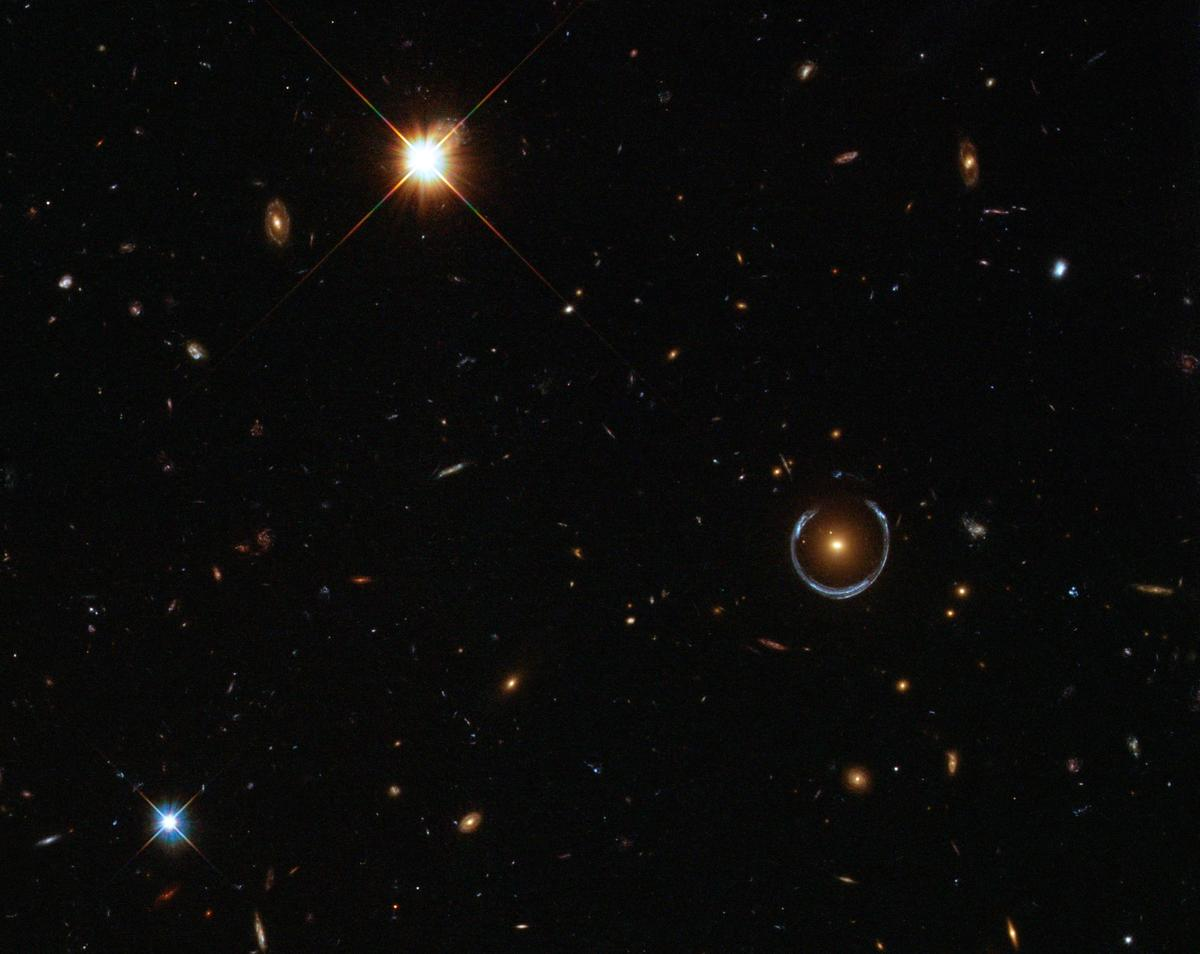
\includegraphics[width=0.85\textwidth]{img/einstein_ring_big.jpg}
\caption{An Einstein ring (Hubble): gravitational lensing effect. In T0, light deflection is coherent phase curvature of the vacuum field. Credit: NASA/ESA Hubble.}
\end{figure}
Newton introduced the gravitational constant~$G$ to make his equation $F = G m_1 m_2 / r^2$ dimensionally consistent. Since then $G$ has been treated as a fundamental constant of nature --- a number that must be measured and is not amenable to deeper explanation.

In the T0 theory this is different. $G$ is not an independent parameter. It follows from~$\xsi$:
\begin{equation}
G = \frac{\xsi^2}{4\,m_e} \times C_{\text{conv}} \times \Kfrak
\end{equation}

This is not a fit. It is a \emph{derivation}. $G$ comes out with the experimentally measured value $G_{\text{SI}} = 6.67 \times 10^{-11}\;\text{m}^3/(\text{kg}\cdot\text{s}^2)$ --- reconstructable from~$\xsi$ alone.

\section{Why Gravity Is So Weak}

The ``weakness'' of gravity --- the fact that it is about~$10^{39}$ orders of magnitude weaker than the electromagnetic force --- is one of the great unsolved puzzles of physics. It is the famous \emph{hierarchy problem}: why is gravity so incredibly weak compared to all other forces?

The answer in T0 is surprisingly simple: $G$ scales as~$\xsi^2$. Since $\xsi \approx 1.33 \times 10^{-4}$, we have $\xsi^2 \approx 1.78 \times 10^{-8}$. The apparent weakness of gravity is nothing other than the fact that $\xsi$ is small --- and $\xsi$ is small because spacetime is almost perfectly three-dimensional ($\Df = 3 - \xsi \approx 2.9999$).

There is no hierarchy problem. There is only a geometric dilution.

\section{The Planck Length as a Geometric Quantity}

From $G$ follows the Planck length. In natural units ($c = \hbar = 1$):
\begin{equation}
\lP = \sqrt{G} = \frac{\xsi}{2\sqrt{m_e}}
\end{equation}

(In SI units $\lP = \sqrt{\hbar G/c^3} \approx 1.616 \times 10^{-35}$~m.)

This is remarkable. The Planck length (cf.\ \href{https://github.com/jpascher/T0-Time-Mass-Duality/blob/main/2/pdf/012_T0_Gravitationskonstante_De.pdf}{Doc.~012}, \href{https://github.com/jpascher/T0-Time-Mass-Duality/blob/main/2/pdf/127_gravitationskonstnte_De.pdf}{127}) --- traditionally the ``smallest meaningful length'' in physics, at which quantum gravity becomes relevant --- is in T0 a purely geometric consequence of~$\xsi$ and the electron mass.

And here a circle closes: the Planck length calculated from the experimentally measured~$G$ agrees \emph{exactly} with the Planck length calculated from~$\xsi$. Why? Because both calculations describe the same geometric reality --- just from different vantage points.

\begin{kerngedanke}
The deeper insight: $G$ encodes the coupling between the $\xsi$-geometry and matter. The gravitational constant does not ``measure'' the strength of a force --- it describes how the torsion of spacetime responds to mass distributions.
\end{kerngedanke}
